\documentclass[12pt]{article}

\usepackage{tikz} 
\usetikzlibrary{shapes}
\usetikzlibrary{arrows}


\usepackage{tikz-cd}
\usetikzlibrary{cd}

\begin{document}


\begin{tikzpicture}
\node (a) at (0,3) {Plam};
\draw (0,0) node (b) {Plim};
\end{tikzpicture}




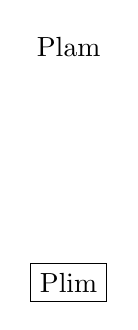
\begin{tikzpicture}
\node (a) at (0,3) {Plam};
\draw (0,0) node
[draw] (b) {Plim};
\end{tikzpicture}



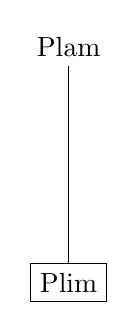
\begin{tikzpicture}
\node (a) at (0,3) {Plam};
\draw (0,0) node
[draw] (b) {Plim};
\draw (a) -- (b);
\end{tikzpicture}



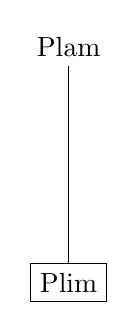
\begin{tikzpicture}
\node (a) at (0,3) {Plam};
\draw (0,0) node
[draw] (b) {Plim};
\draw (a) -- (b);
\end{tikzpicture}



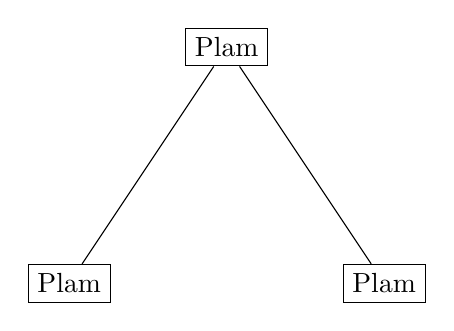
\begin{tikzpicture}
\node[draw] (a) at (2,3) {Plam};
\node[draw] (b) at (0,0) {Plam};
\node[draw] (c) at (4,0) {Plam};
\draw (a) -- (b);
\draw (a) -- (c);
\end{tikzpicture}



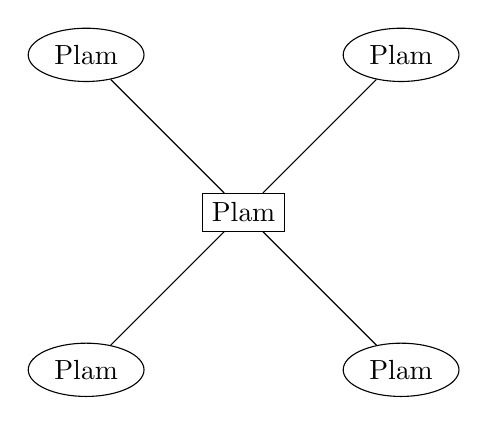
\begin{tikzpicture}
\node[draw] (a) at (2,2) {Plam};
\node[draw,ellipse] (b) at (0,0) {Plam};
\node[draw,ellipse] (c) at (4,0) {Plam};
\node[draw,ellipse] (d) at (0,4) {Plam};
\node[draw,ellipse] (e) at (4,4) {Plam};
\draw (a) -- (b);
\draw (a) -- (c);
\draw (a) -- (d);
\draw (a) -- (e);
\end{tikzpicture}



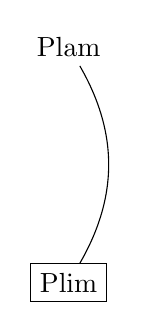
\begin{tikzpicture}
\node (a) at (0,3) {Plam};
\draw (0,0) node
[draw] (b) {Plim};
\draw (a) to [bend left] (b);
\end{tikzpicture}





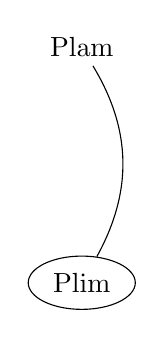
\begin{tikzpicture}
\node (a) at (0,3) {Plam};
\draw (0,0) node
[draw,ellipse] (b) {Plim};
\draw (a) to [bend left] (b);
\end{tikzpicture}





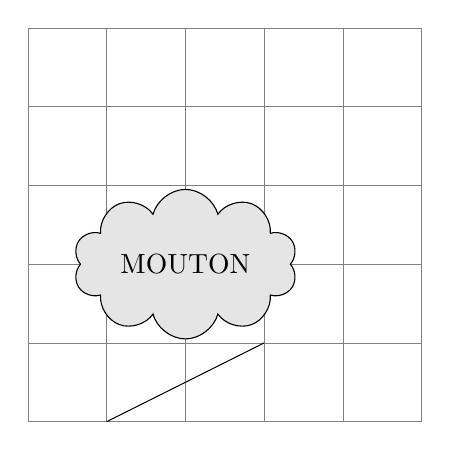
\begin{tikzpicture}
\draw [help lines] (0,0) grid (5,5);
\node [draw,cloud,fill=gray!20,
aspect=2] at (2,2) {MOUTON};
\draw (1,0) -- (3,1) ;
\end{tikzpicture}





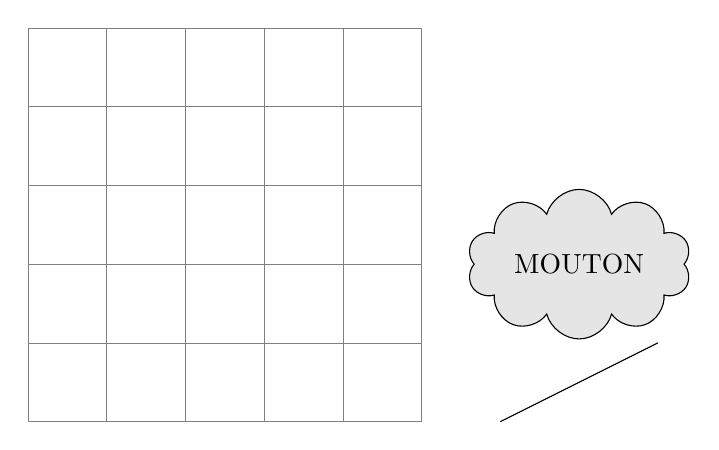
\begin{tikzpicture}
\draw [help lines] (0,0) grid (5,5);
\begin{scope}[xshift=5cm]
\node [draw,cloud,fill=gray!20,
aspect=2] at (2,2) {MOUTON};
\draw (1,0) -- (3,1) ;
\end{scope}
\end{tikzpicture}









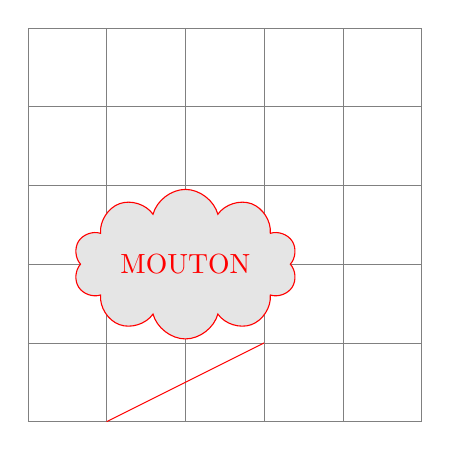
\begin{tikzpicture}
\draw [help lines] (0,0) grid (5,5);
\begin{scope}[red]
\node [draw,cloud,fill=gray!20,
aspect=2] at (2,2) {MOUTON};
\draw (1,0) -- (3,1) ;
\end{scope}
\end{tikzpicture}











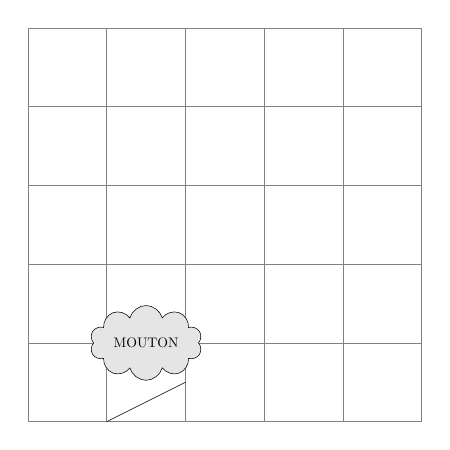
\begin{tikzpicture}
\draw [help lines] (0,0) grid (5,5);
\begin{scope}[xshift=1cm,
transform canvas={scale=.5}]
\node [draw,cloud,fill=gray!20,
aspect=2] at (2,2) {MOUTON};
\draw (1,0) -- (3,1) ;
\end{scope}
\end{tikzpicture}







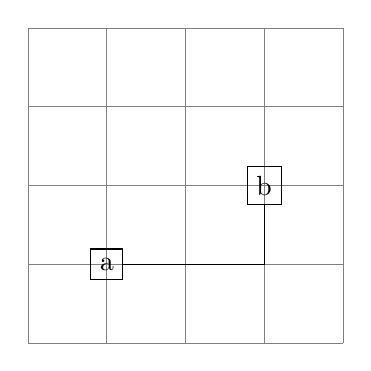
\begin{tikzpicture}
\draw [help lines] (0,0) grid (4,4);
\node[draw] (a) at (1,1) {a};
\node[draw] (b) at (3,2) {b};
\draw (a) -| (b);
\end{tikzpicture}







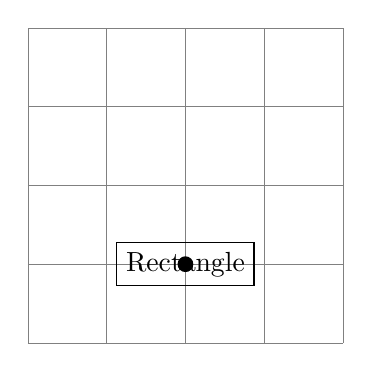
\begin{tikzpicture}
\draw [help lines] (0,0) grid (4,4);
\node[draw] (a) at (2,1) {Rectangle};
\fill (a.center) circle (1mm);
\end{tikzpicture}







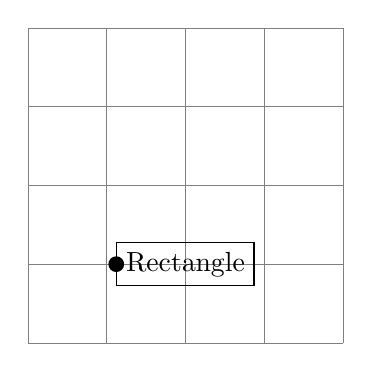
\begin{tikzpicture}
\draw [help lines] (0,0) grid (4,4);
\node[draw] (a) at (2,1) {Rectangle};
\fill (a.west) circle (1mm);
\end{tikzpicture}










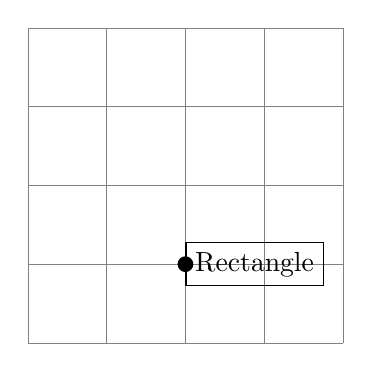
\begin{tikzpicture}
\draw [help lines] (0,0) grid (4,4);
\node[draw,anchor=west] (a)
at (2,1) {Rectangle};
\fill (a.west) circle (1mm);
\end{tikzpicture}










\begin{tikzpicture}
\foreach \i in {0,...,9}
\draw (\i,0) node {\i} ;
\end{tikzpicture}




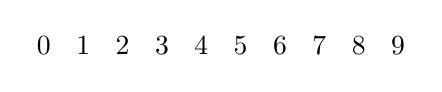
\begin{tikzpicture}
\foreach \i in {0,...,9}
\draw (\i/2,0) node {\i} ;
\end{tikzpicture}






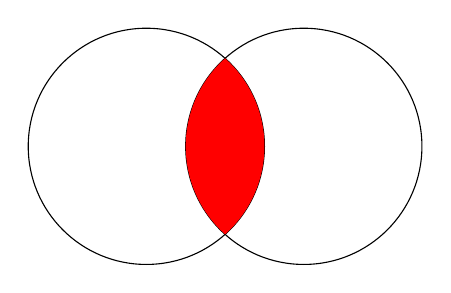
\begin{tikzpicture}
\draw (1,1.5) circle (1.5) ;
\draw (3,1.5) circle (1.5) ;
\clip (3,1.5) circle (1.5) ;
\fill [red] (1,1.5) circle (1.5) ;
\end{tikzpicture}




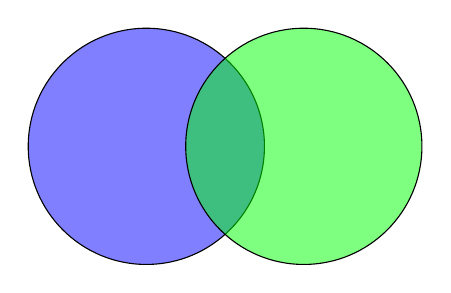
\begin{tikzpicture}
\draw [fill=blue,fill opacity=.5]
(1,1.5) circle (1.5) ;
\draw [fill=green,fill opacity=.5]
(3,1.5) circle (1.5) ;
\end{tikzpicture}








\begin{tikzcd}
A \arrow[rd] \arrow[r, "\phi"] & B \\
                                        & C
\end{tikzcd}



\begin{tikzcd}
A \arrow[r, "\phi"] \arrow[d, red] & B \arrow[d, "\psi" red] \\
C \arrow[r, red, "\eta" blue] & D 
\end{tikzcd}





\begin{tikzcd}
A \arrow[r, "\phi" near start, "\psi"', "\eta" near end] & B
\end{tikzcd}






\begin{tikzcd}[column sep=small]
& A \arrow[dl] \arrow[dr] & \\
B \arrow{rr} & & C
\end{tikzcd}





\begin{tikzcd}[row sep=tiny]
& B \arrow[dd] \\
A \arrow[ur] \arrow[dr] & \\
& C
\end{tikzcd}








\begin{tikzcd}
A \arrow[r, red, shift left=1.5ex] \arrow[r]
\arrow[dr, blue, shift right=1.5ex] \arrow[dr]
& B \arrow[d, purple, shift left=1.5ex] \arrow[d]\\
& C
\end{tikzcd}









\begin{tikzcd}
A \arrow[r]
& B \arrow[r, shift left]
\arrow[r, shift right]
& C \arrow[r]
\arrow[r, shift left=2]
\arrow[r, shift right=2]
& \cdots
\end{tikzcd}







\begin{tikzcd}
A \arrow[r, yshift=0.7ex] \arrow[r, yshift=-0.7ex]
& B \arrow[d, xshift=0.7ex] \arrow[d, xshift=-0.7ex] \\
& C
\end{tikzcd}









\begin{tikzcd}
A \arrow[dr, controls={+(1.5,0.5) and +(-1,0.8)}]
\arrow[dr, dashed, to path=|- (\tikztotarget)]
& \\
& B \arrow[loop right]
\end{tikzcd}












\begin{tikzcd}
A \arrow[r]
& B \arrow[r]
\arrow[d, phantom, ""{coordinate, name=Z}]
& C \arrow[dll,
"\delta",
rounded corners,
to path={ -- ([xshift=2ex]\tikztostart.east)
|- (Z) [near end]\tikztonodes
-| ([xshift=-2ex]\tikztotarget.west)
-- (\tikztotarget)}] \\
D \arrow[r]
& E \arrow[r]
& F
\end{tikzcd}









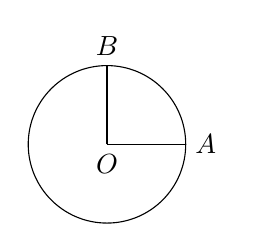
\begin{tikzpicture}
\draw (0,0) -- (1,0) ;
\draw (0,0) -- (0,1) ;
\draw (0,0) circle (1) ;
\draw (0,0) node[below]{$O$} ;
\draw (1,0) node[right]{$A$} ;
\draw (0,1) node[above]{$B$} ;
\end{tikzpicture}









\begin{tikzpicture}
\draw (0,0) node[below] {$O$};
\draw (2,0) node[right] {$A$};
\draw (2,2) node[right] {$B$};
\draw (0,0) -- (2,0) ;
\draw (0,0) -- (2,2);
\draw (1,0) arc (0:45:1) ;
\end{tikzpicture}






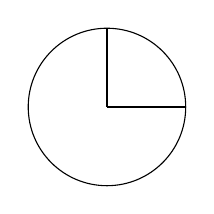
\begin{tikzpicture}
\coordinate (O) at (0,0) ;
\coordinate (A) at (1,0) ;
\coordinate (B) at (0,1) ;
\draw (O) -- (A) ;
\draw (O) -- (B) ;
\draw (O) circle (1) ;
\end{tikzpicture}









\begin{center}
\begin{tikzpicture}
\draw[->] (-1,0) -- (1,0);
\draw (1,0) node[right] {$x$};
\draw [->] (0,-1) -- (0,1);
\draw (0,1) node[above] {$y$};
\end{tikzpicture}
\end{center}








\begin{center}
\begin{tikzpicture}
\draw[->] (-1,0) -- (3,0);
\draw (3,0) node[right] {$x$};
\draw [->] (0,-1) -- (0,3);
\draw (0,3) node[above] {$y$};
\draw [dashed] (2,1) -- (2,0) node[below] {$2$};
\draw [dashed] (2,1) -- (0,1) node[left] {$1$};
\end{tikzpicture}
\end{center}









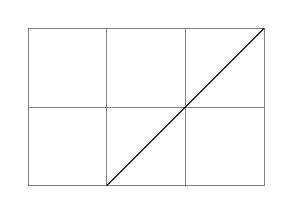
\begin{tikzpicture}
\draw [very thin, gray] (0,0) grid (3,2);
\draw (1,0) -- (3,2);
\end{tikzpicture}






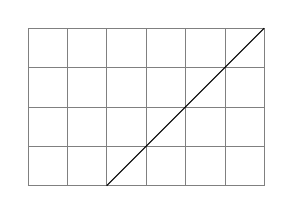
\begin{tikzpicture}
\draw [very thin, gray,step=0.5] (0,0) grid (3,2);
\draw (1,0) -- (3,2);
\end{tikzpicture}







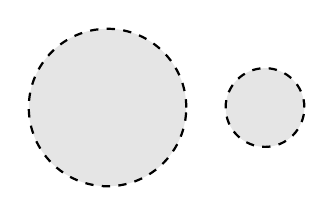
\begin{tikzpicture}
\tikzstyle{grisEncadre}=[thick, dashed, fill=gray!20]
\draw [grisEncadre] (0,0) circle (1);
\draw [grisEncadre] (2,0) circle(0.5);
\end{tikzpicture}











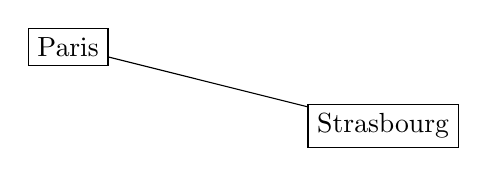
\begin{tikzpicture}
\node[draw] (P) at (0,0) {Paris};
\node[draw] (S) at (4,-1) {Strasbourg};
\draw (P) -- (S);
\end{tikzpicture}





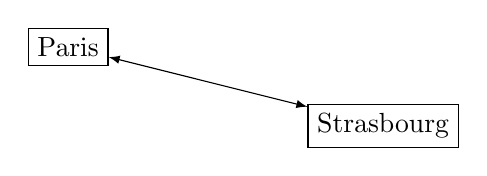
\begin{tikzpicture}
\node[draw] (P) at (0,0) {Paris};
\node[draw] (S) at (4,-1) {Strasbourg};
\draw[<->,>=latex] (P) -- (S);
\end{tikzpicture}









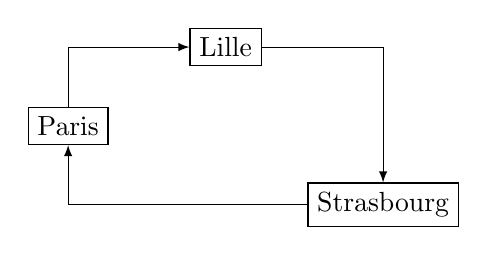
\begin{tikzpicture}
\node[draw] (P) at (0,0) {Paris};
\node[draw] (L) at (2,1) {Lille};
\node[draw] (S) at (4,-1) {Strasbourg};
\draw[->,>=latex] (P) |- (L);
\draw[->,>=latex] (L) -| (S);
\draw[->,>=latex] (S) -| (P);
\end{tikzpicture}









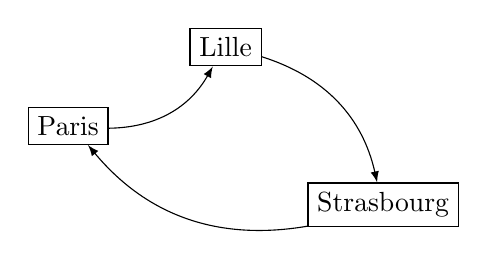
\begin{tikzpicture}
\node[draw] (P) at (0,0) {Paris};
\node[draw] (L) at (2,1) {Lille};
\node[draw] (S) at (4,-1) {Strasbourg};
\draw[->,>=latex] (P) to[bend right] (L);
\draw[->,>=latex] (L) to[bend left] (S);
\draw[->,>=latex] (S) to[bend left] (P);
\end{tikzpicture}







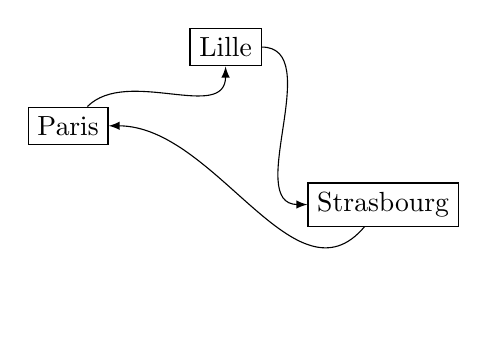
\begin{tikzpicture}
\node[draw] (P) at (0,0) {Paris};
\node[draw] (L) at (2,1) {Lille};
\node[draw] (S) at (4,-1) {Strasbourg};
\draw[->,>=latex] (P) to[out=45,in=-90] (L);
\draw[->,>=latex] (L) to[out=0,in=180] (S);
\draw[->,>=latex] (S) to[out=230,in=0] (P);
\end{tikzpicture}






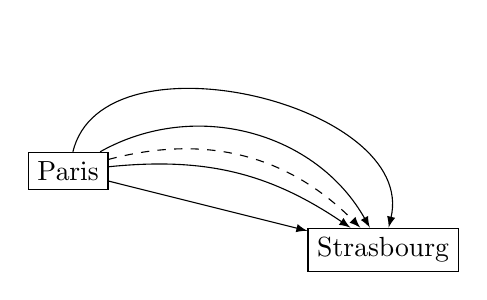
\begin{tikzpicture}
\node[draw] (P) at (0,0) {Paris};
\node[draw] (S) at (4,-1) {Strasbourg};
\draw[->,>=latex] (P) to[bend left=0] (S);
\draw[->,>=latex] (P) to[bend left=20] (S);
\draw[->,>=latex,dashed] (P) to[bend left] (S);
\draw[->,>=latex] (P) to[bend left=45] (S);
\draw[->,>=latex] (P) to[bend left=90] (S);
\end{tikzpicture}












\begin{tikzpicture}
\draw[{[-]}] (0,0) -- (1,1); 
\draw[*-o] (2,0) -- (3,1);
\draw[>->>] (4,0) -- (5,1); 
\draw[)-(] (6,0) -- (7,1);
\draw[|<-)] (8,0) -- (9,1); 
\draw[{]-)}] (10,0) -- (11,1);
\end{tikzpicture}








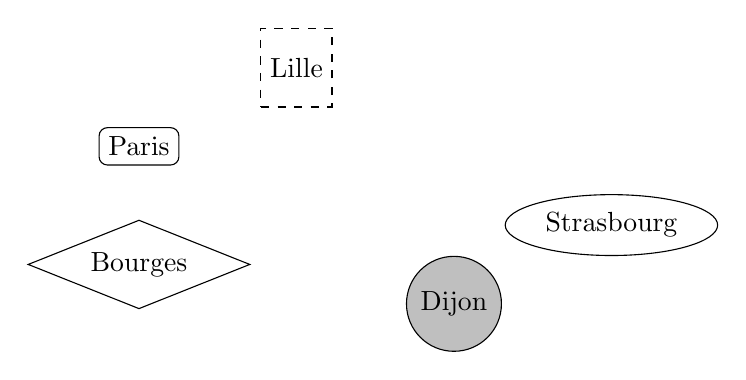
\begin{tikzpicture}
\node[draw,rectangle,rounded corners=3pt] (P)at(0,0){Paris};
\node[draw,minimum height=1cm,dashed] (L)at(2,1) {Lille};
\node[draw,ellipse] (S)at(6,-1) {Strasbourg};
\node[draw,diamond,aspect=2.5] (B)at(0,-1.5) {Bourges};
\node[draw,circle,fill=gray!50] (D)at(4,-2) {Dijon};
\end{tikzpicture}













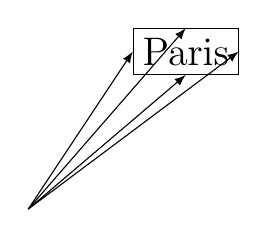
\begin{tikzpicture}
\node[draw] (N) at (2,2) {\Large Paris};
\draw[->,>=latex] (0,0) -- (N.north);
\draw[->,>=latex] (0,0) -- (N.south);
\draw[->,>=latex] (0,0) -- (N.west);
\draw[->,>=latex] (0,0) -- (N.east);
\end{tikzpicture}










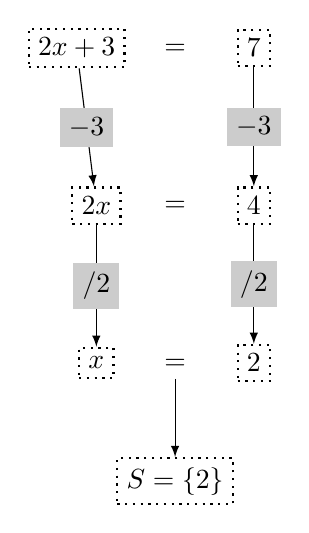
\begin{tikzpicture}
\tikzstyle{membre}= [rectangle,draw,thick,dotted]
\tikzstyle{operation}=[->,>=latex]
\tikzstyle{etiquette}=[midway,fill=black!20]
\node[membre] (g) at (-1.25,4.5) {$2x+3$};
\node[below=-5pt] at (0,4.5) {$=$};
\node[membre] (d) at (1,4.5) {$7$};
\node[membre] (gg) at (-1,2.5) {$2x$};
\node [below=-5pt] at (0,2.5) {$=$};
\node[membre] (dd) at (1,2.5) {$4$};
\node[membre] (ggg) at (-1,0.5) {$x$};
\node [below=-5pt] (egal) at (0,0.5) {$=$};
\node[membre] (ddd) at (1,0.5) {$2$};
\node[membre] (reponse) at (0,-1) {$S=\{2\}$};
%flèches
\draw[operation] (g)--(gg) node[etiquette]{$-3$};
\draw[operation] (d)--(dd) node[etiquette] {$-3$};
\draw[operation] (gg)--(ggg) node[etiquette]{$/2$};
\draw[operation] (dd)--(ddd) node[etiquette] {$/2$};
\draw[operation] (egal)--(reponse);
\end{tikzpicture}











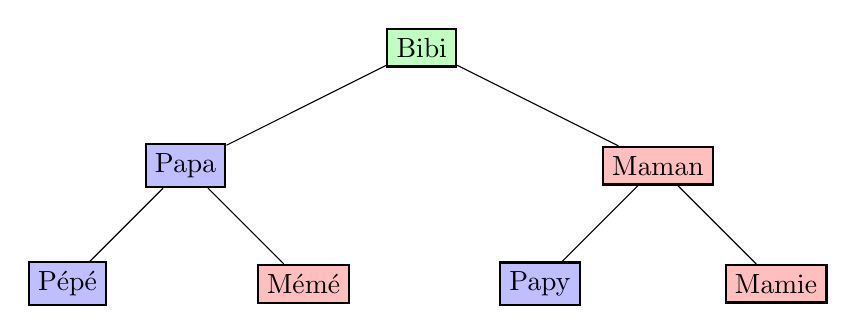
\begin{tikzpicture}
\tikzstyle{lien}=[->,>=stealth,rounded corners=5pt,thick]
\tikzset{individu/.style={draw,thick,fill=#1!25},
individu/.default={green}}
\node [individu] {Bibi} [sibling distance=6cm]
child { node [individu=blue]{Papa} [sibling distance=3cm]
child { node [individu=blue]{Pépé} }
child { node [individu=red]{Mémé} }
}
child { node [individu=red]{Maman} [sibling distance=3cm]
child { node [individu=blue]{Papy} }
child { node [individu=red]{Mamie} }
};
\end{tikzpicture}













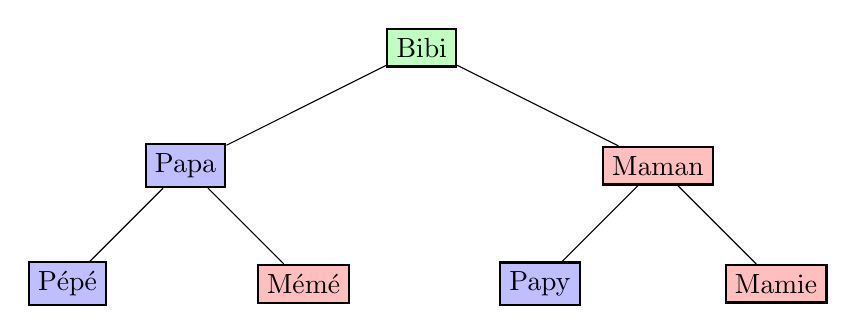
\begin{tikzpicture}[level 1/.style={sibling distance=6cm},
level 2/.style={sibling distance=3cm}]
\tikzstyle{lien}=[->,>=stealth,rounded corners=5pt,thick]
\tikzset{individu/.style={draw,thick,fill=#1!25},
individu/.default={green}}
\node [individu] {Bibi} 
child { node [individu=blue]{Papa} 
child { node [individu=blue]{Pépé} }
child { node [individu=red]{Mémé} }
}
child { node [individu=red]{Maman}
child { node [individu=blue]{Papy} }
child { node [individu=red]{Mamie} }
};
\end{tikzpicture}







\end{document}